%
% Copyright (C) 2011 Agostino De Marco
%                    <agostino dot demarco at unina dot it>
%                    Roberto Giacomelli
%                    <giaconet dot mailbox at gmail dot com>
%
%    This work may be distributed and/or modified under the
%    conditions of the LaTeX Project Public License, either
%    version 1.3 of this license or any later version.
%    The latest version of this license is in
%    http://www.latex-project.org/lppl.txt and version 1.3
%    or later is part of all distributions of LaTeX version
%    2005/12/01 or later.
%
% This work has the LPPL maintenance status `maintained'.
% 
% The Current Maintainer of this work are Agostino De Marco
% and Roberto Giacomelli
%
\documentclass{standalone}
\usepackage{lmodern}
\usepackage{amsmath,fixmath}
\usepackage{relsize}
\usepackage{pgfplots}
\usepackage{pgfplotstable}
\usetikzlibrary{patterns}
\usetikzlibrary{calc}

\usepackage{siunitx}

\begin{document}

\pgfkeys{
   /pgf/number format/.cd,
      use comma
}
\pgfplotsset{
   every axis/.append style={
      font=\relsize{2},
      % very thick,% thick
      % tick style={very thick} % semithick
      line width=1.2pt, % 1.8pt,% thick
      tick style={line width=1.2pt} % 1.8pt semithick
      },
   every axis x label/.append style={
      font=\relsize{4},
      yshift=-6pt,
      xshift=0em
   },
   every axis y label/.append style={
      font=\relsize{3},
      rotate=-90, % -90,
      xshift=0em, % -0.2em,
      yshift=0em, % 0.5em
   },
   major grid style={
      line width = 0.8pt,
      black,
      dash pattern=on 8pt off 4pt
   },
   every axis title/.append style={
      font=\relsize{3}
   }
}

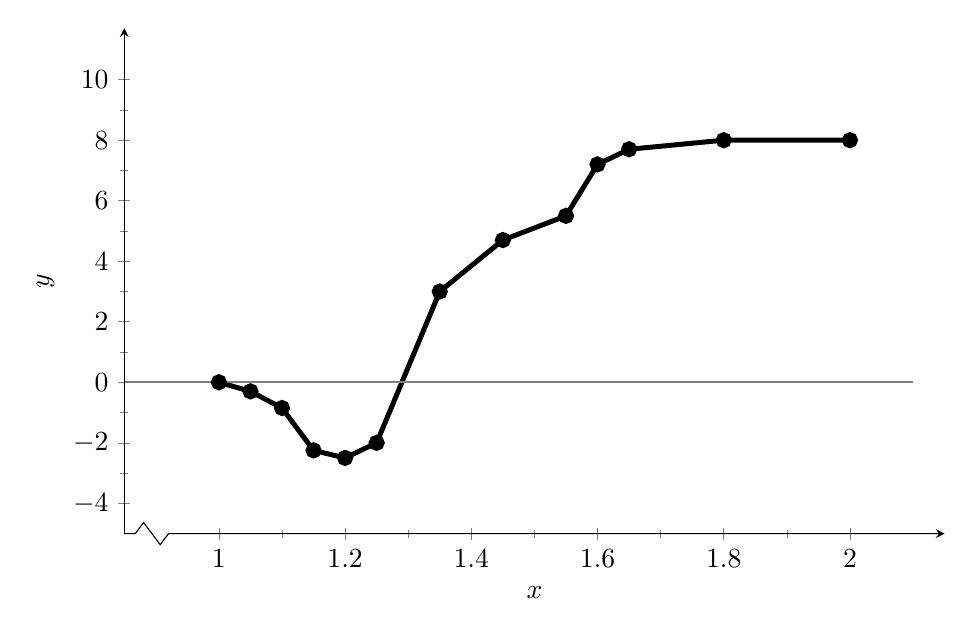
\begin{tikzpicture}
\begin{axis}[
   width=12cm,height=8cm,
   xmin=0.85, xmax=2.15,
   ymin=-5, ymax=11.7,
   xtick={1,1.2,...,2},
   ytick={-4,-2,...,10},
   minor x tick num = 1,
   minor y tick num = 1,
   axis x line=bottom,
   axis y line=left,
   axis x discontinuity=crunch,
   xlabel={$x$},
   ylabel={$y$},
   title={},
   axis on top=true, clip=false
]

\addplot [line width=1.8pt, mark=*] coordinates {
   (1.00,   0.00)
   (1.05, -0.30)
   (1.10, -0.85)
   (1.15, -2.25)
   (1.20, -2.50)
   (1.25, -2.00)
   (1.35,   3.00)
   (1.45,   4.70)
   (1.55,   5.50)
   (1.60,   7.20)
   (1.65,   7.70)
   (1.80,   8.00)
   (2.00,   8.00)
};

\draw [thick,gray] (axis cs: 0.85,0) -- (axis cs: 2.1,0);
\end{axis}
\end{tikzpicture}
\end{document}